\section{Performance evaluation}
\label{section:project_evaluation}

The implementation of the Physarum-based Metaheuristic algorithm is tested under variety of conditions. Some tests have been made to show a general behaviour of the algorithm depending on an input problem size, while other test the influence of various parameters, helping out with their selection. At the end the algorithm is compared to other common algorithms.


\subsection{Dataset description}

The algorithm is tested on QAPLIB dataset library \cite{burkard1997qaplib}. This dataset is \textit{de~facto} standard for testing various Quadratic Assignment Problem solvers. It includes dozens of problem definitions with optimal solutions (or approximations where no optimal solution has been found yet) in an unified format. Some of the inputs are synthetic, generated using various algorithms (i.e. \texttt{lipa} or \texttt{nug}), while some problems are taken from the real world (i.e. \texttt{els} or \texttt{ste}).


\subsection{Testing methodology}

Same seed value has been used across the tests unless mentioned otherwise --- this simple trick ensures the same initial position even if different configuration options are used. Test cases \texttt{lipa20a} and \texttt{lipa90a} are used for testing various parameters as they greatly differ in size ($n=20$ and $n=90$), so influences of the parameters can be observed. Values of observable parameters are measured every epoch (a discrete algorithm step), while the execution time is bounded by a 300~s limit unless mentioned otherwise.

All tests have been done on the same test machine with a given specification: processor Intel Xeon E3-1246 3.5GHz, DDR3-1600 32GB RAM, Linux kernel 3.19. Every plot used in this work is generated automatically (using a Python scripts with \texttt{matplotlib} library) from logs made by \texttt{physarum-debug} (the logs are included with the source). Some detailed numerical values are provided in tables in Appendix \ref{chapter:results}.


\subsection{Colony initialization phase}

The algorithm initialization phase begins with sampling of $k$ random solutions from whole $n!$ search space, then on $l$ best solutions instances of \texttt{Plasmodium} are put. The size of the population directly affects a total number of visited solutions (solutions that were used as food source when plasmodia crawled), larger populations visit more solutions (figure \ref{figure:am_visited_solutions}), because they start in multiple points of the space search. An obvious observation is that introducing more plasmodia results in more computation, as a result each discrete epoch takes longer time to compute --- these experiments were limited to 300~s execution time, larger colonies finished on earlier epochs.

Larger colonies are merging earlier than smaller colonies (figure \ref{figure:am_state_of_colony}), which is an anticipated behaviour --- the chance of encountering another plasmodium is greater as there are more plasmodia sharing the same space search. It can be observed that as a result of merging number of solutions stops increasing drastically as in early epochs, because there are less plasmodia crawling.

\begin{figure}
  \centering

  \begin{subfigure}{\textwidth}
    \includegraphics[width=1.1\textwidth,center]{algorithm/metaheuristic/charts/u/am_visited_solutions_lipa20a.\eop}
    \caption{instance \texttt{lipa20a} $n=20$}
  \end{subfigure}
  \par\bigskip
  \begin{subfigure}{\textwidth}
    \includegraphics[width=1.1\textwidth,center]{algorithm/metaheuristic/charts/u/am_visited_solutions_lipa90a.\eop}
    \caption{instance \texttt{lipa90a} $n=90$}
  \end{subfigure}

  \caption{Number of visited solutions with different colony size $l$ and samples $k$}
  \label{figure:am_visited_solutions}
\end{figure}

\begin{figure}
  \centering

  \begin{subfigure}{\textwidth}
    \includegraphics[width=1.1\textwidth,center]{algorithm/metaheuristic/charts/u/am_state_of_colony_10_30.\eop}
    \caption{population $l=10$, samples $k=30$}
  \end{subfigure}
  \par\bigskip
  \begin{subfigure}{\textwidth}
    \includegraphics[width=1.1\textwidth,center]{algorithm/metaheuristic/charts/u/am_state_of_colony_100_300.\eop}
    \caption{population $l=100$, samples $k=300$}
  \end{subfigure}
  \par\bigskip
  \begin{subfigure}{\textwidth}
    \includegraphics[width=1.1\textwidth,center]{algorithm/metaheuristic/charts/u/am_state_of_colony_300_300.\eop}
    \caption{population $l=300$, samples $k=300$}
  \end{subfigure}

  \caption{State of a colony with a different colony size $l$ and samples $k$ (instance \texttt{lipa90a} $n=90$)}
  \label{figure:am_state_of_colony}
\end{figure}


\begin{figure}
  \centering

  \begin{subfigure}{\textwidth}
    \includegraphics[width=1.1\textwidth,center]{algorithm/metaheuristic/charts/u/am_best_cost_lipa20a.\eop}
    \caption{instance \texttt{lipa20a} $n=20$}
  \end{subfigure}
  \par\bigskip
  \begin{subfigure}{\textwidth}
    \includegraphics[width=1.1\textwidth,center]{algorithm/metaheuristic/charts/u/am_best_cost_nug20.\eop}
    \caption{instance \texttt{nug20} $n=20$}
  \end{subfigure}

  \caption{Cost of the best detected solution by any plasmodium with a different colony size $l$ and samples $k$}
  \label{figure:am_best_cost}
\end{figure}

For small test cases a regularity has been observed --- larger populations tend to find better results in earlier epochs (figure \ref{figure:am_best_cost}). Furthermore, larger $\frac{l}{k}$ proportions (number of plasmodia vs number of samples) are preferred as they exhibit the same characteristic --- when the same number of samples is used, more plasmodia started on these samples yield better results earlier. Plasmodium initialised on a bad solution can crawl towards better one, where a plasmodium initialised on a relatively good solution may not find any better in its local neighbourhood. Thus one should use $l$ close to $k$ to fully use the algorithm potential.


\subsection{Energy values}

Essential parts of the algorithm are $E_{explore}$ and $E_{crawl}$ energy values. The first one has a direct effect on the size of a frontier and number of explored solutions, while the second one has an effect on the size of the plasmodium. Indeed, large values of $E_{explore}$ cause the frontier to be rather small, as few solutions can be explored and added as interesting to the frontier (figure \ref{figure:am_energy_frontier}). On the other hand, larger values of $E_{crawl}$ make plasmodium to occupy less food sources (figure \ref{figure:am_energy_size}).

Moreover there is a latent relation between frontier size and $E_{crawl}$ value --- the frontier size tend to oscillate when $E_{crawl}$ is rather large (figure \ref{figure:am_energy_frontier}), it is so because a plasmodium must conserve the energy for a crawl phase instead of an exploration phase. We also can notice a strong relationship between $E_{explore}$ and cost of the explored best solution (figure \ref{figure:am_energy_cost}) --- small values of $E_{explore}$ tend to visit minimal solutions in earlier epochs.

\begin{figure}
  \centering

  \includegraphics[width=1.1\textwidth,center]{algorithm/metaheuristic/charts/u/am_energy_frontier.\eop}

  \caption{Average size of frontier for colonies with different energies $E_{explore}$ and $E_{crawl}$ (dataset \texttt{lipa20a} $n=20$, $l=10$, $k=30$)}
  \label{figure:am_energy_frontier}
\end{figure}

\begin{figure}
  \centering

  \includegraphics[width=1.1\textwidth,center]{algorithm/metaheuristic/charts/u/am_energy_size.\eop}

  \caption{Average size of plasmodia for colonies with different energies $E_{explore}$ and $E_{crawl}$ (dataset \texttt{lipa20a} $n=20$, $l=10$, $k=30$)}
  \label{figure:am_energy_size}
\end{figure}

\begin{figure}
  \centering

  \includegraphics[width=1.1\textwidth,center]{algorithm/metaheuristic/charts/u/am_energy_cost.\eop}

  \caption{Cost of the best detected solution by any plasmodium with different energies $E_{explore}$ and $E_{crawl}$ (dataset \texttt{lipa20a} $n=20$, $l=10$, $k=30$)}
  \label{figure:am_energy_cost}
\end{figure}

Another parameter that can be used to tune the algorithm is $E_{initial}$ --- initial quanta of energy given to plasmodia on their initialization. Experiments have shown that it has little to none meaning in usual cases. A clear change is visible in the frontier size at the first epoch (figure \ref{figure:am_energy_initial}) --- with bigger $E_{initial}$ there is more energy so more exploration steps can be done (each using $E_{explore}$). In tested cases it has little effect on the solution, however one can imagine a large instance of QAP where a thorough exploration of neighbours on initialization can in fact result in finding close solution to the optimal one at early stages.

\begin{figure}
  \centering

  \includegraphics[width=1.1\textwidth,center]{algorithm/metaheuristic/charts/u/am_energy_initial.\eop}

  \caption{Average frontier size with different initial energy $E_{initial}$ (dataset \texttt{lipa90a} $n=90$, $l=10$, $k=30$)}
  \label{figure:am_energy_initial}
\end{figure}

An unfortunate consequence of the algorithm design is $O(n!)$ space complexity, on a par with $O(n!)$ computation complexity in the worst case (figure \ref{figure:am_energy_spacetime}), however a wise selection of $E_{explore}$ and $E_{crawl}$ energies results in a stricter bounded computations. If every solution is visited, ${\Delta}E_{solution}$ values must be stored $n!$ times, however this is the worst case scenario, rather not likely to happen in practice. Rather small number of solutions are crawled and occupied during work of the program, it would require extremely small $E_{explore}$ values to force the algorithm to occupy every solution, therefore using $O(n!)$ memory and $O(n!)$ computation steps - using sane values of energy averts these adverse effects. As the tests are time-bounded instead of epoch-bounded, a more complex exploration phase results in a lower count of epochs.

\begin{figure}
  \centering

  \begin{subfigure}{\textwidth}
    \includegraphics[width=1.1\textwidth,center]{algorithm/metaheuristic/charts/u/am_energy_spacetime_space.\eop}
    \caption{Memory usage}
  \end{subfigure}
  \par\bigskip
  \begin{subfigure}{\textwidth}
    \includegraphics[width=1.1\textwidth,center]{algorithm/metaheuristic/charts/u/am_energy_spacetime_time.\eop}
    \caption{Total time}
  \end{subfigure}

  \caption{Resources usage with different $E_{explore}$ and $E_{crawl}$ (dataset \texttt{lipa20})}
  \label{figure:am_energy_spacetime}
\end{figure}


\subsubsection{Random walk}

Some combinations of $E_{explore}$ and $E_{crawl}$ can result in a meaningless ``random walk'' and should be avoided. When $E_{explore}$ and $E_{crawl}$ are of a similar value and their sum is close to the unit value (energy of best solution from the sampling phase), plasmodia will choose any solution no matter their energetic value and corresponding cost (figure \ref{figure:am_energy_random}). Such behaviour omits any optimisation behaviour, crawling to solutions without any benefits, hence the name random walk.

\begin{figure}
  \centering

  \includegraphics[width=1.1\textwidth,center]{algorithm/metaheuristic/charts/u/am_energy_random.\eop}

  \caption{Cost of best solution in frontier for every plasmodium with random walk conditions $E_{crawl}=0.3$, $E_{explore}=0.5$ (dataset \texttt{lipa20a} $n=20$, $l=10$, $k=30$)}
  \label{figure:am_energy_random}
\end{figure}

\subsubsection{Plasmodial death}
% TODO plasmodial death

Extreme values of $E_{explore}$ combined with large values $E_{crawl}$ results in a premature plasmodium death. Instead of merging or lasting until the time limit, multiple plasmodia die as they lack energy for crawling to another solution and gaining some new energy (figure \ref{figure:am_energy_death}).

\begin{figure}
  \centering

  \begin{subfigure}{\textwidth}
    \includegraphics[width=1.1\textwidth,center]{algorithm/metaheuristic/charts/u/am_energy_death_5_49.\eop}
    \caption{$E_{explore}=0.5$, $E_{crawl}=0.49$}
  \end{subfigure}
  \par\bigskip
  \begin{subfigure}{\textwidth}
    \includegraphics[width=1.1\textwidth,center]{algorithm/metaheuristic/charts/u/am_energy_death_5_45.\eop}
    \caption{$E_{explore}=0.5$, $E_{crawl}=0.45$}
  \end{subfigure}

  \caption{State of colony with different extreme $E_{explore}$ and $E_{crawl}$ (dataset \texttt{lipa20a} $n=20$, $l=10$, $k=30$)}
  \label{figure:am_energy_death}
\end{figure}


\subsection{Cost to food transformation}

An important step is the cost to food transformation --- each solution's cost is transformed into nutritional energy using equation \ref{equation:m_e_solution}. Every solution is compared to the best solution from the sampling phase, every quotient $\frac{calibrated\_cost}{cost(solution)}$ is amplified using the exponential function with the base $q$, linearly scaled using a coefficient $a$ (usually $a=q^{-1}$).

Using such transformation gives solutions equal to the best sample an unit value of $E_{solution}=1$, worse solutions carry lower energy, while better solutions carry bigger energy. Modifying the base $q$ (and a corresponding scale $a$) can be used to intensify this difference.

\begin{figure}
  \centering

  \includegraphics[width=1.1\textwidth,center]{algorithm/metaheuristic/charts/u/am_ctf_food.\eop}

  \caption{Plasmodium energy $E_{plasmodium}$ with different base $q$ and scale $a$ (dataset \texttt{lipa20a} $n=20$, $l=1$, $k=10$)}
  \label{figure:am_ctf_food}
\end{figure}

\begin{figure}
  \centering

  \includegraphics[width=1.1\textwidth,center]{algorithm/metaheuristic/charts/u/am_ctf_frontier.\eop}

  \caption{Size of frontier with different base $q$ and scale $a$ (dataset \texttt{lipa20a} $n=20$, $l=1$, $k=10$)}
  \label{figure:am_ctf_frontier}
\end{figure}

Experiments confirm that larger $q$ values provide more energy to plasmodia (figure \ref{figure:am_ctf_food}) as explored solution carry more $E_{solution}$ energy. This extra energy is used for exploration phase and result in larger frontier sizes (figure \ref{figure:am_ctf_frontier}).


\subsection{Optimization results}

In order to assess usefulness of the Physarum-based Metaheuristic algorithm two measures are used: a relative distance to an optimal solution and an assignment similarity measure. The relative distance is defined as follows:
\begin{equation}
  dist(cost, optimum) = \frac{cost - optimum}{optimum}
\end{equation}
Where $cost$ is the cost of compared solution and $optimum$ is the cost of the optimal arrangement (or its best known approximation) given as input data from \texttt{QAPLIB}. With such a measure values closer to $0.0$ are preferred, as they are closer to the optimal cost.

The similarity measure aggregates differences in the assignment to a simple real value. The similarity is defined as fraction of assignments on the same position:
\begin{equation}
  sim(a, b) = \frac{| x : a(x) = b(x), x \in [1, n] \subset \mathbb{N}|}{|n|}
\end{equation}
Where $a$ and $b$ are compared assignment and $n$ is the problem size. This measure is defined between 0 and 1, with $sim(a, b) = 0$ meaning complete mismatch and $sim(a, b) = 1$ meaning complete match. One should notice that an assignment can be optimal ($dist=0$), even though its $sim(a, opt) \leq 1$ --- multiple assignments can yield the same optimal cost.

The first experiments have been done on \texttt{lipa} dataset, which is made of 8 different problem definitions of size $n \in \{20, 30, 40, 50, 60, 70, 80, 90\}$. An universal values of $E_{explore}=0.001$ and $E_{crawl}=0.01$, scaling factor $a=0.1$, exponential base $q=10$, population size $l=100$ out of $k=300$ samples, time of execution was made relative to input size $t=4n$.

\begin{figure}
  \centering

  \begin{subfigure}{0.47\textwidth}
    \includegraphics[width=1.0\textwidth]{algorithm/metaheuristic/charts/complipaoriginal/distance.eps}
    \caption{Distance to the optimal solution}
  \end{subfigure}
  \begin{subfigure}{0.47\textwidth}
    \includegraphics[width=1.0\textwidth]{algorithm/metaheuristic/charts/complipaoriginal/similarity.eps}
    \caption{Similarity with optimal assignment}
  \end{subfigure}

  \caption{Results for \texttt{lipa} dataset}
  \label{figure:am_lipa_results}
\end{figure}

Obtained results (figure \ref{figure:am_lipa_results}) look promising, but are not truly satisfactory. For small instances a relative error is quite large, even though most of the assignment is the same as the optimal assignment. A conclusion can be made, that plasmodium is close to the solution, however it might have missed it or crawled out of it. Furthermore, for larger instances there is almost no similarity between computed and the optimal assignment, even though a relative distance is acceptable ($dist < 1\%$) --- the plasmodia have crawled into a local minima far from optimal neighbourhood.

\subsubsection{Improved algorithm}

A solution for this sub-efficient behaviour has been quickly found. In earlier evaluations of the algorithm (figure \ref{figure:am_best_cost}), we observed that plasmodia can crawl out of optimal solutions. This behaviour is a result of plasmodia avoiding being stuck in a local optimum, however it has no knowledge if the optimum is local or a global minimum.

At this point a minor improvement to the algorithm has been added --- each plasmodium stores the best solution it explored during its lifetime. This does not change a behaviour of the plasmodium, it just adds another observation of the plasmodial behaviour. While original algorithm returned the best occupied solution by any plasmodium, the improved algorithm returns the best solution ever found by any plasmodium.

\begin{figure}
  \centering

  \begin{subfigure}{0.9\textwidth}
    \includegraphics[width=1.0\textwidth]{algorithm/metaheuristic/charts/complipaimproved/distance.eps}
    \caption{Distance to the optimal solution}
  \end{subfigure}
  \begin{subfigure}{0.9\textwidth}
    \includegraphics[width=1.0\textwidth]{algorithm/metaheuristic/charts/complipaimproved/similarity.eps}
    \caption{Similarity with optimal assignment}
  \end{subfigure}

  \caption{Results for \texttt{lipa} dataset for original and improved algorithm}
  \label{figure:am_lipa_results_improved}
\end{figure}

As predicted this change made a positive influence on the results (figure \ref{figure:am_lipa_results_improved}). For \texttt{lipa20a} and \texttt{lipa30a} the optimal assignment have been found, where for other instances of \texttt{lipa}, assignments worse only by less than $1~\%$ from the optimum cost have been found. Furthermore the improved implementation has been tested with longer execution time $t=10n$ instead $t=4n$, which has given slightly better results. The improved version of the algorithm provides better results and it will be used for further tests.


\subsubsection{QAPLIB results}

Using generic parameters (population $l=100$, samples $k=300$, $E_{explore}=0.001$, $E_{crawl}=0.01$, exponential base $q=10$ and scale $a=0.1$), tests for every case in \texttt{QAPLIB} have been done. Every test has been repeated ten times, no random seed has been preset as it is a practical test. Results are aggregated in different ways --- by minimum cost (showing the best case) and by average cost presenting an usual result for given dataset. Every instance has been allowed to run for time $t=10n$, but no longer than 900~s. Results from these tests are aggregated in \Crefrange{figure:am_qaplib_result:bur}{figure:am_qaplib_result:tai}, detailed data in tabular form are available in Appendix \ref{chapter:results}.

\newcommand{\qaplibresultchart}[1]{
  \begin{figure}
    \centering

    \begin{subfigure}{0.47\textwidth}
      \includegraphics[width=1.0\textwidth]{algorithm/metaheuristic/charts/multiple/#1/distance.eps}
      \caption{Distance to the optimal solution}
    \end{subfigure}
    \begin{subfigure}{0.47\textwidth}
      \includegraphics[width=1.0\textwidth]{algorithm/metaheuristic/charts/multiple/#1/similarity.eps}
      \caption{Similarity with optimal assignment}
    \end{subfigure}

    \caption{Aggregated results for \texttt{#1} dataset}
    \label{figure:am_qaplib_result:#1}
  \end{figure}
}

\qaplibresultchart{bur}
\qaplibresultchart{chr}
\qaplibresultchart{had}
\qaplibresultchart{lipaa}
\qaplibresultchart{lipab}
\qaplibresultchart{nug}
\qaplibresultchart{rou}
\qaplibresultchart{scr}
\qaplibresultchart{sko}
\qaplibresultchart{tai}

From the obtained results we can conclude that our algorithm, with proposed settings, works satisfactory well for most of the problems, especially when instance size is relatively small $n<40$. In such cases the cost is usally less than $1\%$ worse than the optimal solution, multiple times the optimal assignment has been found (datasets \texttt{bur}, \texttt{had}, \texttt{lipa}, \texttt{nug}, \texttt{rou} and \texttt{scr}). Furthermore in some cases, the proposed assignment, even though it bares the optimal cost, it is a different one than the one proposed by the authors of \texttt{QAPLIB} --- such behaviour can be observed in \texttt{had14}, \texttt{had16} (figure \ref{figure:am_qaplib_result:had}), \texttt{nug15} (figure \ref{figure:am_qaplib_result:nug}) and others.

Two datasets \texttt{chr} and \texttt{lipab} can be considered unusually difficult for the algorithm, yielding rather poor results. An explanation for \texttt{lipab} is a usage of very large numbers in the weight matrix, unfortunately the default cost to food transform cannot represent these values effectively, some further research on selecting $a$ and $q$ might be needed to solve this case efficiently. As for \texttt{chr} the distance matrix is very sparse and the algorithm struggles with finding useful random neighbours.


\subsubsection{Optimising large instances}

Solving large QAP is especially practical and indeed requires usage of heuristic methods. For such large instances of $n>50$, the number of possible arrangements is unimaginable. Our algorithm gives acceptable results for many large inputs like \texttt{lipa80a}, \texttt{lipa90a} (figure \ref{figure:am_qaplib_result:lipaa}) with distance of less than $1\%$, or whole \texttt{sko} dataset where average distance is less than $2.5\%$ (figure \ref{figure:am_qaplib_result:sko}).

However there are some testcases where the approximated assignment is far from being optimal: \texttt{tai100b} ($dist>7\%$), \texttt{tai150b} ($dist>15\%$) or \texttt{tai256c} ($dist>6\%$). For such cases, generic parameters of the algorithm are not suitable and some more work on their selection muse be done.

As the space search of such problems is huge, used number of samples $k=300$ is too small to be practical, causing the population to be initialized on very unefficient solutions. We can confirm this, as no merges occur during run of the algorithm, thus each plasmodium must occupy far solutions from each other. Some experiments with different number of samples $k$ and population size $l$ have been done (figure \ref{figure:am_tai_frontier}).

\begin{figure}
  \centering

  \includegraphics[width=1.1\textwidth,center]{algorithm/metaheuristic/charts/u/am_tai_frontier.\eop}

  \caption{Cost of the best detected solution by any plasmodium with different initial sample size on large nontrivial dataset \texttt{tai150} $n=150$}
  \label{figure:am_tai_frontier}
\end{figure}

Selecting a larger number of samples $k=3000000$ improves results dramatically --- from initial $dist>15\%$ to much better $dist{\approx}2\%$. It should be noticed that even this number of samples is relatively small compared to size of search spaces, when $n=150$ (in case of \texttt{tai150}) only about $10^{-250}$ space search is sampled.

Some more research should be done before using the Physarum-based Metaheuristic for optimizing real world large instances of QAP, especially when the optimum is not known beforehand. It is recommended to use a large number of samples $k$ and give the algorithm long time limit $t$. For such big instances, obtaining result even after whole day of computations is usually worth the effort.

\subsection{Final results}

% TODO cite
We have compared our algorithm to some industry leading solutions such as \textit{ANGEL}, ant colony, simulated annealing, \textit{GRASP} and MILP \cite{TODO}. While some works are lacking of results for some datasets, a comparison of a distance to the optimal solution can be seen in table \ref{table:result_comparison_distance}, while exact costs of the resulting assignment are visible in table \ref{table:result_comparison_cost}.

\begin{table}
  \centering
  \caption{Comparison of distance to optimal solution using different methods \cite{tseng2006hybrid, karami2013analysis, ramakrishnan1998tight, maniezzo1999ant}}
  \label{table:result_comparison_distance}

  \pgfplotstabletypeset[
    col sep=comma,
    fixed,
    precision=3,
    every col no 0/.style={
      string type,
      column type=r|
    },
    every col no 1/.style={
      dec sep align
    },
    every col no 2/.style={
      dec sep align
    },
    every col no 3/.style={
      dec sep align
    },
    every col no 4/.style={
      dec sep align
    },
    every col no 5/.style={
      dec sep align
    },
    every col no 6/.style={
      dec sep align
    },
    every col no 7/.style={
      column type=|c
    },
    every head row/.style={before row=\toprule,after row=\midrule},
    every last row/.style={after row=\bottomrule}
  ]{resultsdist.csv}
\end{table}

\begin{table}
  \centering
  \caption{Cost obtained using various methods \cite{tseng2006hybrid, karami2013analysis, ramakrishnan1998tight, maniezzo1999ant}}
  \label{table:result_comparison_cost}

  \pgfplotstabletypeset[
    col sep=comma,
    fixed,
    precision=0,
    every col no 0/.style={
      string type,
      column type=r
    },
    every col no 1/.style={
      column type=c|
    },
    every col no 2/.style={
      dec sep align
    },
    every col no 3/.style={
      dec sep align
    },
    every col no 4/.style={
      dec sep align
    },
    every col no 5/.style={
      dec sep align
    },
    every col no 6/.style={
      dec sep align
    },
    every col no 7/.style={
      dec sep align,
      column type/.add={}{|}
    },
    every col no 8/.style={
      column type={c},
      dec sep align
    },
    every head row/.style={before row=\toprule,after row=\midrule},
    every last row/.style={after row=\bottomrule}
  ]{results.csv}
\end{table}

Based on this comparison, we can observe that our algorithm is beaten only by \textit{ANGEL}, but only in little number of cases. This method is a complex hybrid algorithm based on a genetic programming, ant colonies and the local optimization and is a popular choice for solving practical QAP instances. Mixed-integer linear programming gives the same results as our method (however it was tested only for a few cases), but in pracice it is very resource consuming as the whole field of mathematical programming. Other methods are relatively far from the optimum assignment when compared to the proposed algorithm.

Furthermore, we have not found any data on behaviour of other algorithms on especaily large QAP instances. We have shown, that the algorithm being a main matter for this thesis can approximate assignments for large instances in relatively short time. We conclude that with some further parameters tweaking, the same results as leading \textit{ANGEL} method could be obtained. It is important to remember that when using the Physarum-based Metaheuristic algorithm, one should always test a few combinations of configuration parameters in order to tune it well.
